\section{DEMO}

\addcontentsline{lof}{figure}{Demo}

\textbf{Nghiệp vụ của khách hàng:}

\textTo{Khách hàng truy cập website sẽ hiển thị danh sách các tour}

\begin{figure}[ht]
    \centering
    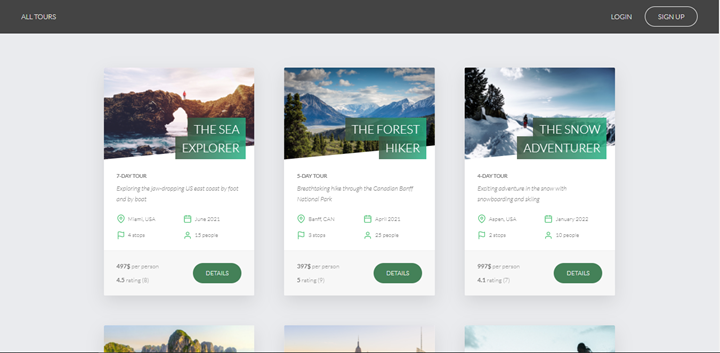
\includegraphics[width = 1.2\linewidth]{figures/demo/1.png}
    \caption{Hình ảnh danh sách tour.}
    \label{fig:example_1}
\end{figure}

\vspace{10cm}

\textTo{Khách hàng chọn xem chi tiết tour}

\begin{figure}[ht]
    \centering
    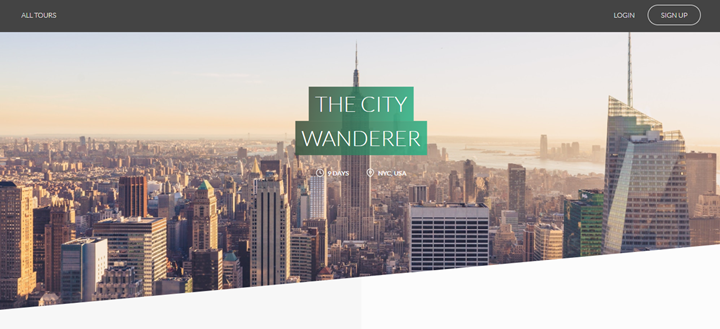
\includegraphics[width = 1.2\linewidth]{figures/demo/2.png}
    \label{fig:example_1}
\end{figure}
\begin{figure}[ht]
    \centering
    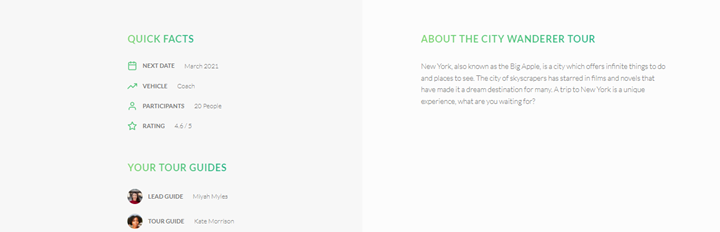
\includegraphics[width = 1.2\linewidth]{figures/demo/3.png}
    \caption{Chi tiết tour.}
    \label{fig:example_1}
\end{figure}

\vspace{15cm}

\textTo{Xem bản đồ chi tiết về ngày, nơi đến.}


\begin{figure}[ht]
    \centering
    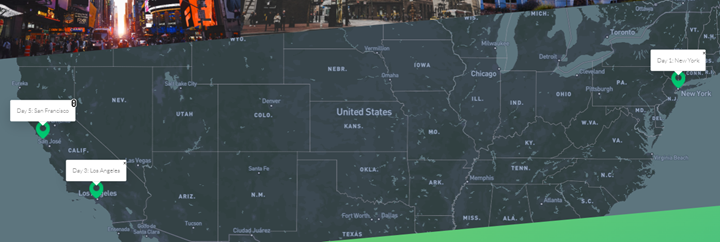
\includegraphics[width = 1.2\linewidth]{figures/demo/bando.png}
    \caption{Bản đồ chi tiết về ngày và nơi đến.}
    \label{fig:example_1}
\end{figure}

\textTo{Xem đánh giá từ các người đã đi tour này}

\begin{figure}[ht]
    \centering
    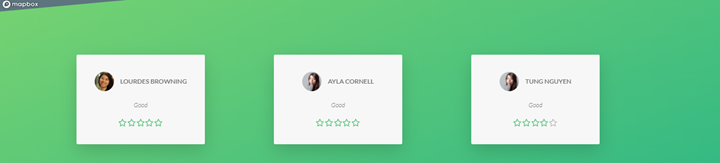
\includegraphics[width = 1.2\linewidth]{figures/demo/5.png}
    \caption{Xem đánh giá từ các người đã đi tour này.}
    \label{fig:example_1}
\end{figure}

\vspace{10cm}

\textTo{Khách hàng sẽ thấy button đặt tour phía dưới cùng, Khách hàng sẽ được yêu cầu đăng nhập để đặt tour}

\begin{figure}[ht]
    \centering
    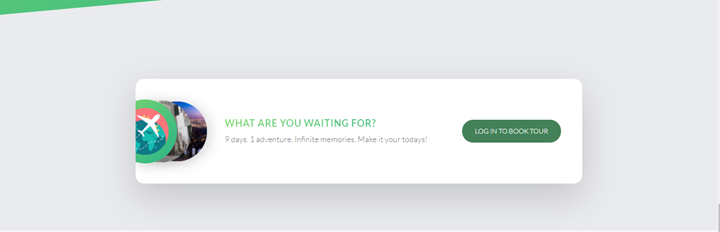
\includegraphics[width = 1.2\linewidth]{figures/demo/6.png}
    \caption{Button đặt tour.}
    \label{fig:example_1}
\end{figure}

\textTo{Nếu khách hàng chưa có tài khoản thì sẽ được phép đăng ký tài khoản mới}

\begin{figure}[ht]
    \centering
    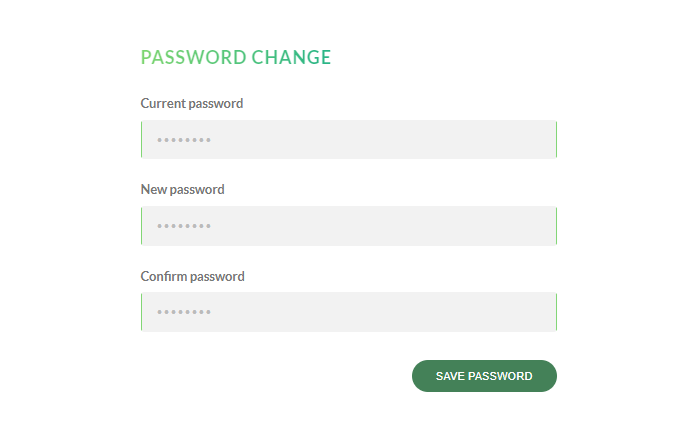
\includegraphics[width = 1\linewidth]{figures/demo/11.png}
    \caption{Đăng ký tài khoảng mới.}
    \label{fig:example_1}
\end{figure}

\vspace{10cm}

\textTo{Sau khi đăng ký thành công thì Khách hàng sẽ nhận được thư qua gmail}

\begin{figure}[ht]
    \centering
    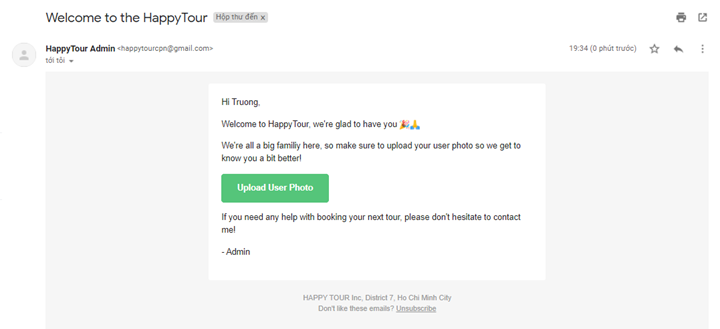
\includegraphics[width = 1\linewidth]{figures/demo/mail.png}
    \caption{Mail xác nhận.}
    \label{fig:example_1}
\end{figure}

\begin{figure}[ht]
    \centering
    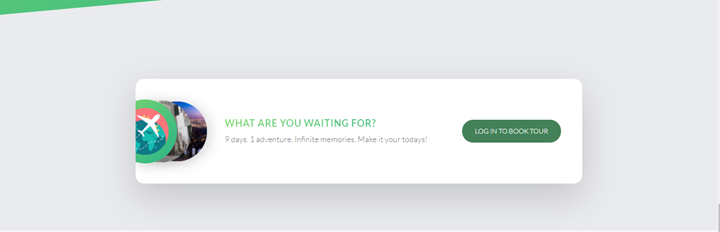
\includegraphics[width = 1\linewidth]{figures/demo/6.png}
    \caption{Button đăng ký tài khoản.}
    \label{fig:example_1}
\end{figure}

\textTo{Sau khi click vào button sẽ chuyển đến trang thanh toán cho khách hàng}

\vspace{10cm}

\textTo{Các thông tin thanh toán được hiển thị đầy đủ}

\begin{figure}[ht]
    \centering
    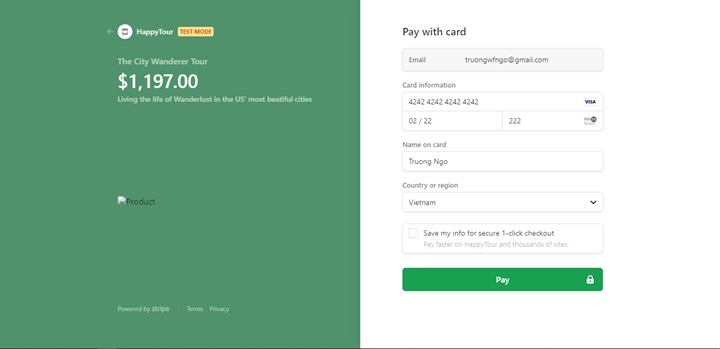
\includegraphics[width = 1\linewidth]{figures/demo/pay.png}
    \caption{Trang thanh toán.}
    \label{fig:example_1}
\end{figure}

\textTo{Phía hê thống sẽ tiếp nhận và xử lý gửi hóa đơn cho khách hàng qua email}

\begin{figure}[ht]
    \centering
    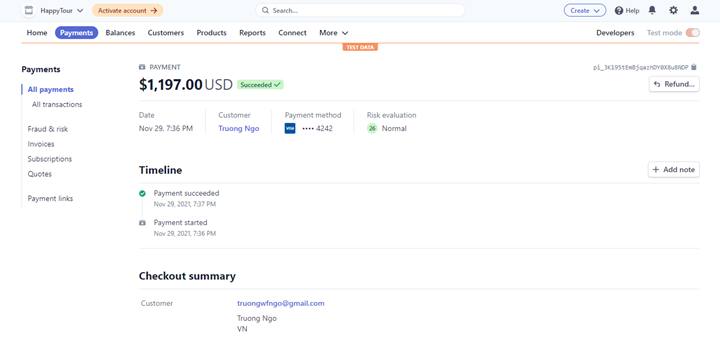
\includegraphics[width = 1\linewidth]{figures/demo/pay1.png}
    \caption{Trang thanh toán.}
    \label{fig:example_1}
\end{figure}

\textTo{Các chức năng ở phần hệ thống quản lí đã làm được hết các API chưa hoành thành bên fronEnd để dựng trang admin}

\begin{figure}[ht]
    \centering
    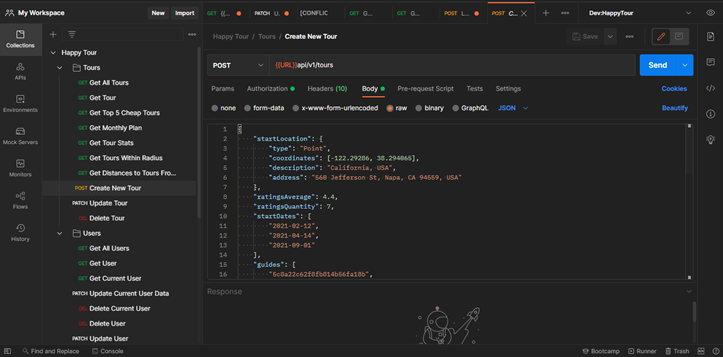
\includegraphics[width = 1\linewidth]{figures/demo/api.png}
    \caption{Trang thanh toán.}
    \label{fig:example_1}
\end{figure}

\vspace{10cm}

\section{Kết luận}

Báo Cáo đã đạt được các yêu cầu cần thiết
\subsection{Phần đồ án:}
\begin{itemize}
\item Hoàn thành các chức năng về nghiệp vụ của khách hàng đã dựng lên web thành công
\item Các chức năng quản lí nội bộ vẫn ở mức API (hoàn thành) chưa triển khai lên trang admin
\item Thiếu các chức năng của kế toán và bộ phận CSKH
\end{itemize}



